\documentclass[12pt, oneside]{article}
\usepackage[letterpaper, margin=1in]{geometry}
\usepackage[english]{babel}
\usepackage[utf8]{inputenc}
\usepackage{amsmath}
\usepackage{amsfonts}
\usepackage{amssymb}
\usepackage{tikz}
%\usepackage{tkz-fct}
\usepackage{pgfplots}
\pgfplotsset{width=10cm,compat=1.9}
\usepgfplotslibrary{statistics}
\usepackage{pgfplotstable}
%\usepackage{venndiagram}

\usepackage{fancyhdr}
\pagestyle{fancy}
\fancyhf{}
\rhead{\thepage \\Name: \hspace{1.5in}}
\lhead{BECA / Dr. Huson / 11.1 IB Math SL\\* 3 May 2018 \\*\textbf{Classwork: Exponential functions\\*
}}

\renewcommand{\headrulewidth}{0pt}

\begin{document}


%\subsection*{Solve equations}

%Solve for the value of $x$.

\begin{enumerate}


\item The function $p(t)=110e^{0.03922t}$ models the population of a city, in millions, $t$ years after 2010.
\begin{enumerate}
    \item Initially, as of 2010, what is the population in millions.\\[40pt]
    \item What is the rate that the population increases continuously, per year?\\[40pt]
    \item Express the population as a function with the form $p(t)=Ab^{t}$, where $A$ and $b$ are real numbers.\\[40pt]
\end{enumerate}

\item For a given time, $x$, in seconds, an electric current, $y$, can be represented by $y = 2.7^{-.10x}$. 
\begin{enumerate}
    \item Simplify the expression to eliminate the coefficient in the exponent.\\[40pt]
    \item Is the electric current increasing or decreasing? Justify your answer.\\[70pt]
    \item Is the current in the original equation, above, exponential growth or decay? Why?\\[70pt]
\end{enumerate}

\newpage

\item Iridium-192 is an isotope of iridium and has a half-life of 73.83 days. If a laboratory experiment begins with 100 grams of Iridium-192, the number of grams, $A$, of Iridium-192 present after $t$ days would be 
\[A=100 \left( \frac{1}{2} \right)^\frac{t}{73.83}\]

\begin{enumerate}
    \item Simplify the equation to eliminate the fraction in the exponent.\\[30pt]
    \item After one day, how much isotope is present?\\[30pt]
    \item As a percentage, how much does the mass of the isotope change each day?\\[30pt]
\end{enumerate}

\item A bank account earns interest at a continuous interest rate of 5\% per year. The initial deposit is \$225.
\begin{enumerate}
    \item Express the balance in the account as a function in the form $P(t)=P_0 \cdot e^{rt}$\\[30pt]
    \item Convert the function to one without a coefficient in the exponent. \\[30pt]
    \item What is the interest rate expressed as a simple, annual rate?\\[30pt]
\end{enumerate}

\item Judith puts \$5000 into an investment account with interest compounded continuously. What is the approximate annual rate is needed for the account to grow to \$9110 after 30 years?

\newpage

\subsection*{Homework}

\item Write $\sqrt[3]x^2$ as a single term with a rational exponent.\\*[30pt]

\item Write $\sqrt{a^2} \div a^3$ as an expression with positive, integer exponents.\\*[30pt]

\item If $n=\sqrt{a^3}$ and $m=a$, where $a > 0$, express $\frac{n}{m}$ as 
\begin{enumerate}
    \item a radical with positive, integer exponents\\*[30pt]
    \item an expression with a fractional exponent\\*[30pt]
\end{enumerate}
\item What is the expression $6xi^3(-4xi+5)$ is equivalent to?\\*[30pt]  %Alg2 Regents Jun2017 multiple choice

\item Simplify the expression $(3k - 2i)^2$, where $i$ is the imaginary unit.\\[30pt] %Alg2 Regents Aug2017

\item Nicole tried to find the product of $(2+ 4i)$ and $(3 - i)$, and her work is shown below.
$(2 + 4i)(3 - i)$\\*
$=6 - 2i + 12i - 4i^2$\\*
$=6 + 10i - 4i^2$\\*
$=6 + 10i - 4(1)$\\*
$=6 + 10i - 4$\\*
$=2 + 10i$\\*
Identify the error in the process shown and determine the correct product of $(2+ 4i)$ and $(3 - i)$.%Alg2 Regents Jan2018
\newpage
\item Graph the function $f(x)=x^3-9x+2$. 
\begin{enumerate}
    \item Write down the $y$-intercept.\\*[10pt]
    \item Mark the $x$-intercepts on the graph as ordered pairs, rounding to the nearest hundredth.\\*[10pt]
\end{enumerate}

\begin{figure}[!ht]
    \centering
    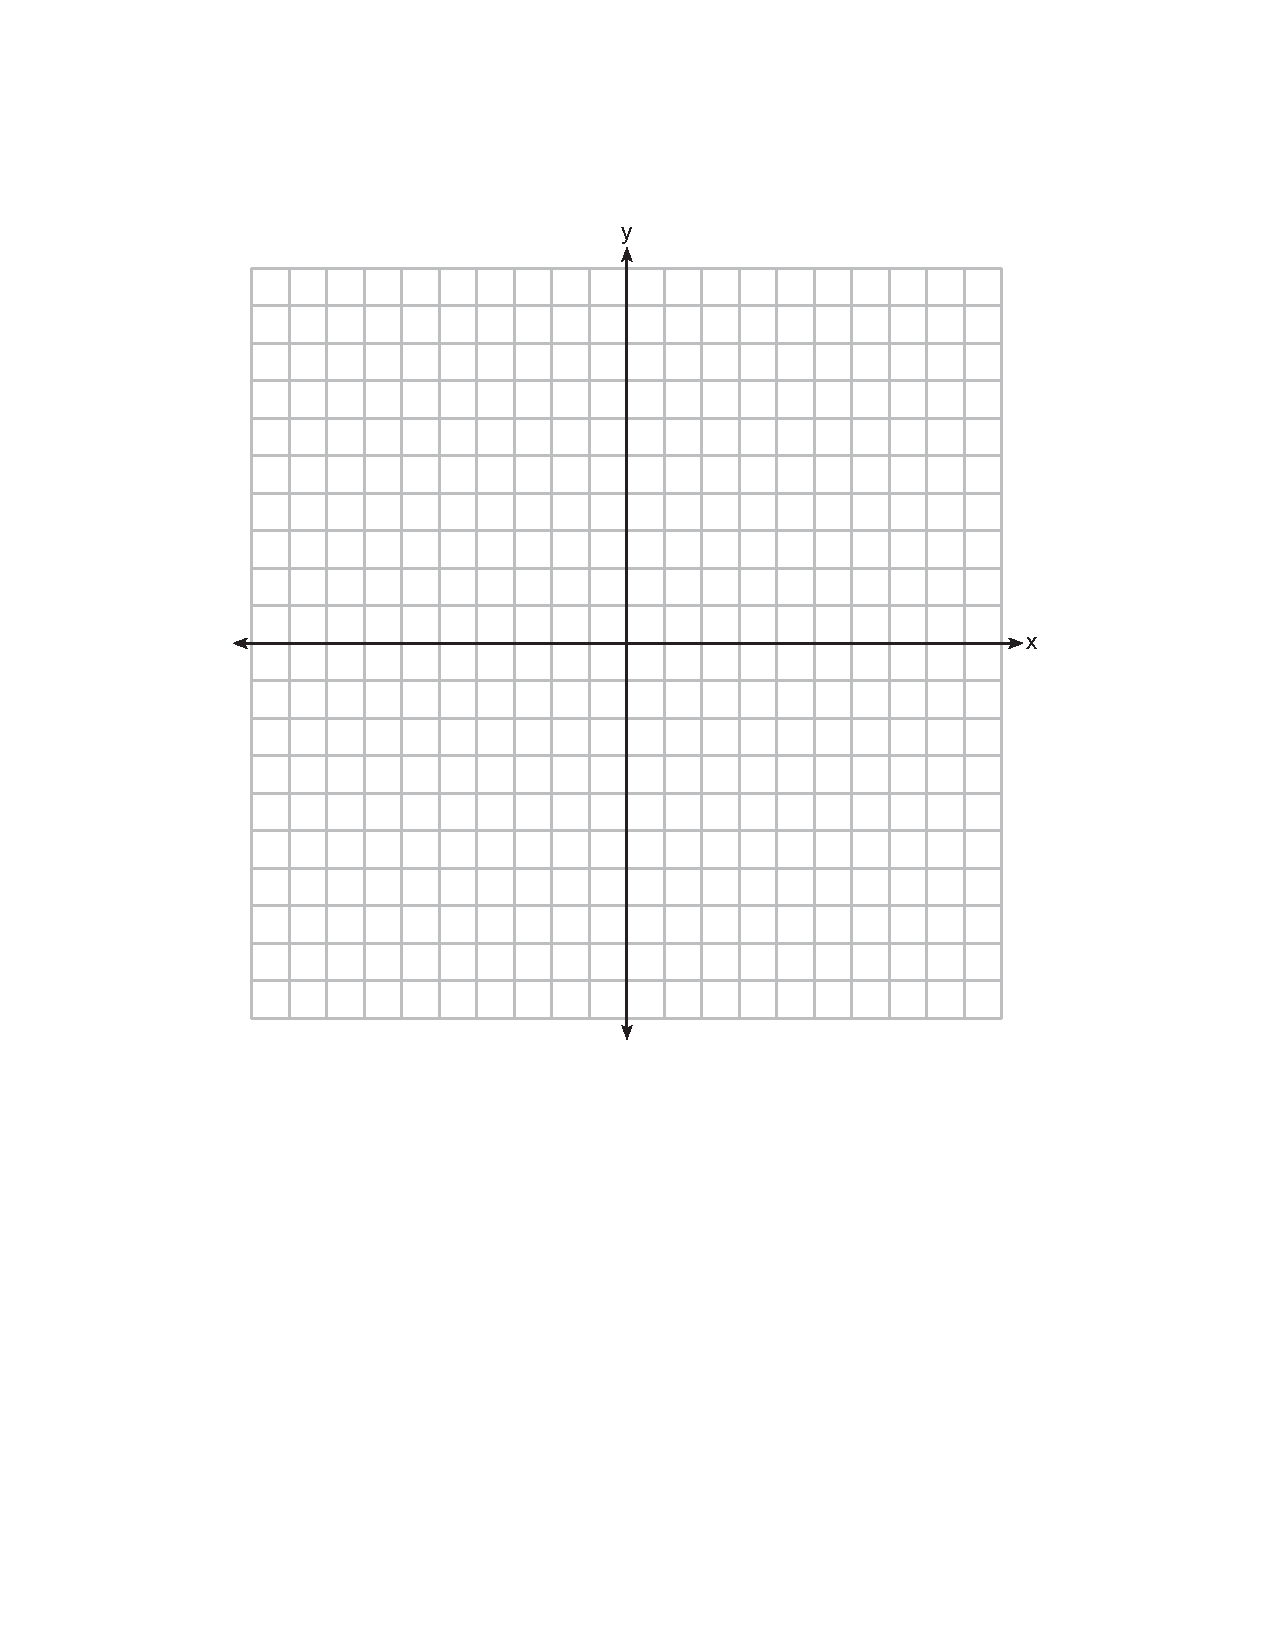
\includegraphics[width=0.75\textwidth]{regents-grid.pdf}
\end{figure}

\item Judith puts \$1000 into an investment account with interest compounded continuously. What is the approximate annual rate is needed for the account to grow to \$1529.59 after 10 years?


\end{enumerate}
\end{document}